\section{Ordinary Least Squares}
This section will introduce the method of ordinary least squares for estimating parameters in a multiple linear regression model.

% \subsection{Least Squares}
% The main idea behind the least squares is to minimize the sum of squared residuals, also known as SSR. 
% Given a set of data points in the plane how might one find the line that best fit the data. 
% One way is to choose the line that minimizes the sum of squared residuals.
% In figure \ref{fig:example_simple_linear_regression} an example of a simple linear regression can be seen. 
% The figure illustrates the log price plotted against the age of property sold by Home in Aalborg within the year 2012.

% \begin{figure}[h]
%     \centering
%     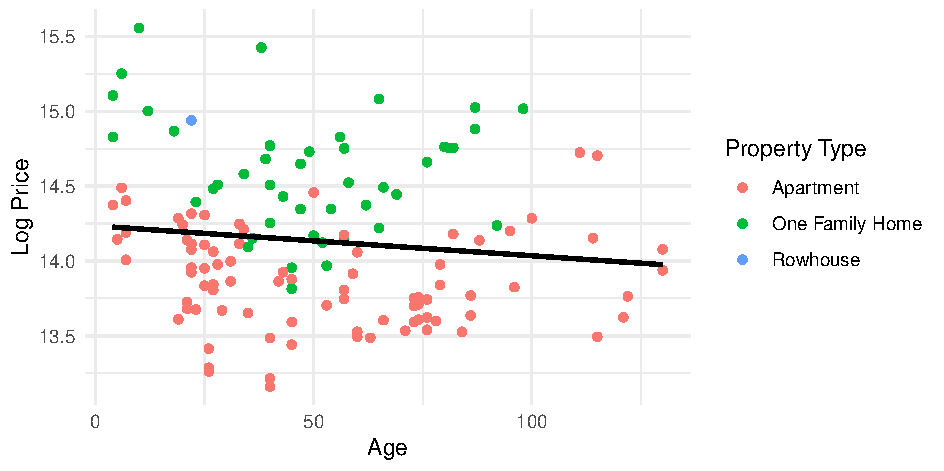
\includegraphics[width = 0.9\textwidth]{figures/Ordinary_Least_Squares/example_linear_regression.pdf}
%     \caption{Age and log price of property sold in 2012 by Home in Aalborg.}
%     \label{fig:example_simple_linear_regression}
% \end{figure}

% The dataset has observations of the form $\{a_i, log(p_i)\}$ with $i = 1, \ldots, 130$. The age of property is seen as the independent variable and the log price as the dependent variable.
% We can assume, albeit naive considering figure \ref{fig:example_simple_linear_regression}, that there is a linear relationship between age and log price of the property in question.
% This can be formulated as
% \begin{align}\label{eq:approx_linear_relationship}
%     \log(p) \approx \beta_0 + \beta_1 a
% \end{align}
% where $log(p)$ and $a$ denotes the log price and age respectively.
% The right side \eqref{eq:approx_linear_relationship} is the model function in our case.
% The function is on the form $f(a, \boldsymbol{\beta})$, where $\boldsymbol{\beta}$ is a $2 \times 1$ vector containing the parameters $\beta_0$ and $\beta_1$.
% The goal is now to find $\boldsymbol{\beta}$ that minimizes the sum of squared residuals.
% For the $i$'th observation the residual is defined as $r_i = log(p_i) - f(a, \boldsymbol{\beta})$.
% With the notation in place we can now write the sum of squared residuals as
% \begin{align}\label{eq:SSR}
%   \ssr(\boldsymbol{\beta}) = \sum_{i = 1}^{130} r_i^2 = \sum_{i = 1}^{130} \left( log(p_i) - f(a, \boldsymbol{\beta}) \right)^2
% \end{align}

\subsection{Parameter Estimation in Matrix Form}
Estimating parameters for a multiple linear regression model in matrix form still translates to minimizing the sum of squared residuals.
The sum of squared residuals now take the form
\begin{align*}
    \ssr(\mathbf{b}) = \nsum (y_i - \mathbf{x}_i\mathbf{b})^2.
\end{align*}
% where $y_i$ denotes the price of property $i$ and $\mathbf{x}_i$ denotes the $i$'th row in the design matrix $\mathbf{X}$.
Where $\mathbf{x}_i$ denotes the $i$'th row in the design matrix $\mathbf{X}$, it is therefore a row vector of the form
\begin{align*}
    \mathbf{x}_i = \begin{bmatrix} 1 & x_{i1} & \cdots & x_{ik} \end{bmatrix}.
\end{align*}
Suppose that $\betahat$ minimizes the sum of squared residuals, that is
\begin{align*}
    \betahat = \underset{\mathbf{b}}{\argmin} \nsum (y_i - \mathbf{x}_i\mathbf{b})^2.
\end{align*}
Where arg is the argument that minimizes the SSR w.r.t.$\!$ $\textbf{b}$. Then $\betahat$ must satisfy the condition $\nabla \ssr(\betahat) = 0$.
Taking the derivative w.r.t. $\mathbf{b}$ yields
\begin{align}\label{eq:ssr_derivative}
    \frac{\partial \ssr(\mathbf{b})}{\partial \mathbf{b}} 
    =  \nsum -2(y_i - \mathbf{x}_i \mathbf{b})\mathbf{x}_i
\end{align}
The expression $\nabla \ssr (\betahat) = 0$ can now be rewritten as
\begin{align*}
    \nsum -2(y_i - \mathbf{x}_i \betahat)\mathbf{x}_i = \mathbf{0} 
    \quad \Rightarrow \quad
    \nsum \mathbf{x}_i^\top(y_i - \mathbf{x}_i \betahat) = \mathbf{0}
\end{align*}
by taking the transpose and dividing by $-2$.
The condition is now a vector of size $(k + 1) \times 1$ and thus represents a system of $k + 1$ equations with $k + 1$ unknowns.
Writing the vector as a system of equations gives the following $k + 1$ equations
\begin{align}\label{eq:multiple_linear_regression_equations}
\begin{split}
    \nsum (y_i - \betahat_0 -  \mathbf{x}_{i1} \betahat_1 - \cdots - \betahat_k \mathbf{x}_{ik}) &= 0 \\
    \nsum \mathbf{x}_{i1}(y_i - \betahat_0 -  \mathbf{x}_{i1} \betahat_1 - \cdots - \betahat_k \mathbf{x}_{ik}) &= 0 \\
    &\vdots \\
    \nsum \mathbf{x}_{ik}(y_i - \betahat_0 -  \mathbf{x}_{i1} \betahat_1 - \cdots - \betahat_k \mathbf{x}_{ik}) &= 0
\end{split}
\end{align}
Returning to the notation used in \eqref{eq:multiple_linear_regression_model}, \eqref{eq:multiple_linear_regression_equations} will now be rewritten to matrix notation
\begin{align}
    \mathbf{X}^\top(\mathbf{y} - \mathbf{X}\betahat) &= \mathbf{0} \nonumber\\
    \mathbf{X}^\top\mathbf{y} - \mathbf{X}^\top\mathbf{X}\betahat &= \mathbf{0}\nonumber\\
    \mathbf{X}^\top\mathbf{X}\betahat &= \mathbf{X}^\top\mathbf{y}\label{eq:equation_from} \\
    \betahat &= \left(\mathbf{X}^\top\mathbf{X}\right)^{-1}\mathbf{X}^\top\mathbf{y}.\label{eq:equation_to}
\end{align}
Going from \eqref{eq:equation_from} to \eqref{eq:equation_to} one must assume that $\mathbf{X}^\top\mathbf{X}$ is positive definite and thereby invertible.
It turns out that this is not the only assumption we have to make, there are in fact five assumptions related to the OLS estimator.
These assumptions will now be listed.
\begin{assumption}[Linear in parameters]\label{as:linear_in_the_parameters}
    The model can be written as $\mathbf{y} = \mathbf{X}\boldsymbol{\beta} + \boldsymbol{\varepsilon}$ where $\mathbf{y}$ is an observed $n \times 1$ vector, $\mathbf{X}$ is an $n \times (k + 1)$ observed matrix, and $\boldsymbol{\varepsilon}$ is an $n \times 1$ vector of unobserved errors or disturbances \cite[p. 809]{Wooldridge2012}.
\end{assumption}
\begin{assumption}[No perfect collinearity]\label{as:no_perfect_collinearity}
    The matrix $\mathbf{X}$ has rank $(k + 1)$ \cite[p. 810]{Wooldridge2012}.
\end{assumption}
As the design matrix $\mathbf{X}$ has $n$ rows and $k + 1$ columns, assumption \ref{as:no_perfect_collinearity} implies that $n \geq k + 1$.
Moreover it implies that $\mathbf{X}$ has full column rank and thereby that $\mathbf{X}^\top\mathbf{X}$ is positive definite.
To prove this consider an arbitrary matrix $X$ of size $m \times n$.
The matrix $(X^\top X)$ is symmetric and positive semi definite, as for any $v \in \mathbb{R}^n$
\begin{align}\label{eq:positive_semi_definite}
v^\top (X^\top X) v = (v^\top X^\top) (X v) = (X v)^\top (X v) \geq 0.
\end{align}
Assume now that $X$ has rank $n$ and for contradiction that $v^\top X v = 0$.
By \eqref{eq:positive_semi_definite} this is a contradiction as it would imply that $vX = 0$ which cannot be true for a matrix of full column rank.
This is because a matrix of full column rank has columns that are linearly independent.
Thus it is proven that if $X$ has full column rank then $X^\top X$ is positive definite.
\begin{assumption}[Zero conditional mean]\label{as:zero_conditional_mean}
    Conditional on the entire matrix $\mathbf{X}$, each error $\varepsilon_i$ has zero mean, i.e. \cite[p. 810]{Wooldridge2012}
    \begin{align*}
        E(\varepsilon_i | \mathbf{X}) = 0, \quad i = 1, 2, \ldots, n.
    \end{align*}
\end{assumption}
This assumption ensures that there is no correlation between each of the explanatory variables and $\varepsilon_i$ for $i = 1, \ldots, n$.
If it on the other hand was the case that $x_j$ were correlated with $\varepsilon_i$, the explanatory variable would be called an endogenous explanatory variable.
In the case that assumption \ref{as:zero_conditional_mean} holds and thereby that none of the explanatory variables are correlated with $\varepsilon_i$, we have what is called exogenous explanatory variables.
\begin{theorem}[Unbiasedness of OLS]
    Under assumptions \ref{as:linear_in_the_parameters}, \ref{as:no_perfect_collinearity} and \ref{as:zero_conditional_mean}, the OLS estimator $\betahat$ is unbiased for $\boldsymbol{\beta}$ \cite[p. 810]{Wooldridge2012}.
\end{theorem}\label{th:unbiasedness_of_ols}
\begin{proof}
    Under assumptions \ref{as:linear_in_the_parameters} and \ref{as:no_perfect_collinearity} we can write $\betahat$ as
    \begin{align}
        \betahat &= (\mathbf{X}^\top\mathbf{X})^{-1}\mathbf{X}^\top\mathbf{y} \nonumber\\
        &= (\mathbf{X}^\top\mathbf{X})^{-1}\mathbf{X}^\top(\mathbf{X}\boldsymbol{\beta} + \boldsymbol{\varepsilon}) \nonumber\\
        &=(\mathbf{X}^\top\mathbf{X})^{-1}\mathbf{X}^\top\mathbf{X}\boldsymbol{\beta} + (\mathbf{X}^\top\mathbf{X})^{-1}\mathbf{X}^\top\boldsymbol{\varepsilon} \nonumber\\
        &= \boldsymbol{\beta} + (\mathbf{X}^\top\mathbf{X})^{-1}\mathbf{X}^\top\boldsymbol{\varepsilon} \label{eq:beta_hat_unbiased}
    \end{align}
    Taking the expectation of \eqref{eq:beta_hat_unbiased} and using the fact that $E(\boldsymbol{\varepsilon} | \mathbf{X}) = 0$ gives that
    \begin{align*}
        E(\betahat | \mathbf{X}) &= \boldsymbol{\beta} + (\mathbf{X}^\top\mathbf{X})^{-1}\mathbf{X}^\top E(\boldsymbol{\varepsilon} | \mathbf{X}) \\
        &= \boldsymbol{\beta} + (\mathbf{X}^\top\mathbf{X})^{-1}\mathbf{X}^\top \mathbf{0} \\
        &= \boldsymbol{\beta}
    \end{align*}
    It is now shown that $\betahat$ is unbiased as defined in definition \ref{def:Unbiased_estmator} on page \pageref{def:Unbiased_estmator}.
\end{proof}
To derive the variance-covariance matrix for the OLS estimator we need to make an assumption regarding the variance of the error term.
\begin{assumption}[Homoskedasticity and no serial correlation]\label{as:homoskedasticity_and_no_serial_correlation}
    This assumption has two parts, the first part, regarding homoskedasticity states that
    \begin{align*}
       \var(\varepsilon_i | \mathbf{X}) = \sigma^2, \quad i = 1,2, \ldots, n.
    \end{align*}
    The second part, regarding serial corellation, states that
    \begin{align*}
        \cov(\varepsilon_i, \varepsilon_j | \mathbf{X}) = 0, \quad \text{for all} \ i \neq j.
    \end{align*}
    In matrix form these to assumptions together becomes
    \begin{align*}
        \var(\boldsymbol{\varepsilon} | \mathbf{X}) = \sigma^2\mathbf{I}_{n\times n}.
    \end{align*}
\end{assumption}
With the previous assumption in place we are now able to derive the variance-covariance matrix of the OLS estimator.
\begin{theorem}[Variance-Covariance Matrix of the OLS Estimator]\label{th:variance-covariance_of_the_ols_estimator}
    Under assumptions \ref{as:linear_in_the_parameters}, \ref{as:no_perfect_collinearity}, \ref{as:zero_conditional_mean} and \ref{as:homoskedasticity_and_no_serial_correlation} the conditional variance of $\betahat$ on $\mathbf{X}$ satisfies \cite[p. 811]{Wooldridge2012} 
    \begin{align*}
        \var(\betahat | \mathbf{X}) = \sigma^2(\mathbf{X}^\top\mathbf{X})^{-1}.
    \end{align*}
\end{theorem}
\begin{proof}
    From \eqref{eq:beta_hat_unbiased} we have
    \begin{align}
        \var(\betahat | \mathbf{X}) &= \var\left[ (\mathbf{X}^\top\mathbf{X})^{-1}\mathbf{X}^\top\boldsymbol{\varepsilon}|\mathbf{X} \right] \nonumber\\
        &= (\mathbf{X}^\top\mathbf{X})^{-1}\mathbf{X}^\top\left[ \var(\boldsymbol{\varepsilon} | \mathbf{X}) \right] \mathbf{X}(\mathbf{X}^\top\mathbf{X})^{-1}, \label{eq:conditional_variance_of_epsilon}
    \end{align}
    and we can now use assumption \ref{as:homoskedasticity_and_no_serial_correlation} to substitute $\var(\boldsymbol{\varepsilon}|\mathbf{X})$ for $\left[\sigma^2 \mathbf{I}\right]$ in \eqref{eq:conditional_variance_of_epsilon} which gives
    \begin{align*}
        \var(\betahat | \mathbf{X}) &= (\mathbf{X}^\top\mathbf{X})^{-1}\mathbf{X}^\top\left[\sigma^2 \mathbf{I}\right] \mathbf{X}(\mathbf{X}^\top\mathbf{X})^{-1} \\
        &= \sigma^2(\mathbf{X}^\top\mathbf{X})^{-1}\mathbf{X}^\top \mathbf{X}(\mathbf{X}^\top\mathbf{X})^{-1} \\
        &= \sigma^2(\mathbf{X}^\top\mathbf{X})^{-1}
    \end{align*}
\end{proof}
As it was explained in conjunction with defintion \ref{def:minimum_mean_square_error}, on page \pageref{def:minimum_mean_square_error}, the BLUE is the estimator that have the smallest variance.
It is possible to establish conditions that any linear unbiased estimator must satisfy, these conditions can then be used to find an expression for the variance of any linear unbiased estimator.
Thus we can compare the variance of the OLS estimator and of any linear unbiased estimator.
This is the motivation for the following theorem.
\begin{theorem}[Gauss-Markov Theorem]
    Under assumptions \ref{as:linear_in_the_parameters}, \ref{as:no_perfect_collinearity}, \ref{as:zero_conditional_mean} and \ref{as:homoskedasticity_and_no_serial_correlation} 
    \begin{align*}
        \betahat &= (\mathbf{X}^\top\mathbf{X})^{-1}\mathbf{X}^\top\mathbf{y}
    \end{align*}
    is the best linear unbiased estimator \cite[p. 811]{Wooldridge2012}.
\end{theorem}\label{th:gauss_markoc_theorem}
\begin{proof}
    Any linear estimator can be written as
    \begin{align}\label{eq:any_linear_operator}
        \boldsymbol{\Tilde{\beta}} = \mathbf{A}^\top \mathbf{y},
    \end{align}
    where $\mathbf{A}$ is an $n \times (k + 1)$ matrix.
    For the linear estimator to be unbiased conditional on $\mathbf{X}$ it must satisfy
    \begin{align}\label{eq:condition_of_unbiasedness}
        E(\betatilde|\mathbf{X}) = \boldsymbol{\beta}.
    \end{align}
    Following that $\mathbf{y} = \mathbf{X}\boldsymbol{\beta} + \boldsymbol{\varepsilon}$ the expectation of $\betatilde$ conditional on $\mathbf{X}$ can be written as
    \begin{align}
       E(\betatilde|\mathbf{X}) &= E( \mathbf{A}^\top\mathbf{X}\boldsymbol{\beta} + \mathbf{A}^\top\boldsymbol{\varepsilon}|\mathbf{X} )\nonumber \\
        &=  \mathbf{A}^\top\mathbf{X}\boldsymbol{\beta} + E( \mathbf{A}^\top\boldsymbol{\varepsilon}|\mathbf{X} )\nonumber \\
        &=\mathbf{A}^\top\mathbf{X}\boldsymbol{\beta} +  \mathbf{A}^\top E( \boldsymbol{\varepsilon}|\mathbf{X} )\nonumber \\
        &=\mathbf{A}^\top\mathbf{X}\boldsymbol{\beta}\label{eq:expectation_of_any_linear_unbiased_estimator}
    \end{align}
    For the linear estimator to be unbiased it must be that \eqref{eq:expectation_of_any_linear_unbiased_estimator} is equal to the left side of \eqref{eq:condition_of_unbiasedness}, as below
    \begin{align}\label{eq:unbiasedness_identity}
        \mathbf{A}^\top\mathbf{X}\boldsymbol{\beta} = \boldsymbol{\beta}
    \end{align}
    The relation in \eqref{eq:unbiasedness_identity} holds if and only if $\mathbf{A}^\top\mathbf{X} = \mathbf{I}_{k + 1}$, which furthermore implies that $(\mathbf{A}^\top\mathbf{X})^\top = \mathbf{X}^\top\mathbf{A} = \mathbf{I}_{k + 1}$.
    The variance of $\betatilde$ conditional on $\mathbf{X}$ is given by
    \begin{align}
        \var(\betatilde|\mathbf{X}) &= \var(\mathbf{A}^\top\mathbf{X}\boldsymbol{\beta} + \mathbf{A}^\top\boldsymbol{\varepsilon}|\mathbf{X}) \nonumber\\
        &= \var(\mathbf{A}^\top\mathbf{X}\boldsymbol{\beta}|\mathbf{X}) + \var(\mathbf{A}^\top\boldsymbol{\varepsilon}|\mathbf{X}) + 2 \cov\left(\mathbf{A}^\top\mathbf{X}\boldsymbol{\beta},\mathbf{A}^\top\boldsymbol{\varepsilon}|\mathbf{X}\right) \nonumber\\
        &= \var(\mathbf{A}^\top\boldsymbol{\varepsilon}|\mathbf{X}) \nonumber\\
        &= \mathbf{A}^\top\var(\boldsymbol{\varepsilon}|\mathbf{X})\mathbf{A}.\label{eq:variance_of_betatilde_conditional_on_x}
    \end{align}
    From assumption \ref{as:homoskedasticity_and_no_serial_correlation} and \eqref{eq:variance_of_betatilde_conditional_on_x} we conclude that
    \begin{align}
        \var(\betatilde|\mathbf{X}) = \sigma^2\mathbf{A}^\top\mathbf{A}
    \end{align}
    Knowing the variance of any linear unbiased estimator we can now subtract the known variance of the OLS estimator, which was found in theorem \ref{th:variance-covariance_of_the_ols_estimator}
    \begin{align}
        \var(\betatilde|\mathbf{X}) - \var(\betahat|\mathbf{X}) &= \sigma^2\mathbf{A}^\top\mathbf{A} - \sigma^2(\mathbf{X}^\top\mathbf{X})^{-1} \nonumber \\
        &= \sigma^2\left[\mathbf{A}^\top\mathbf{A} - (\mathbf{X}^\top\mathbf{X})^{-1} \right] \label{eq:subtraction_of_variances1} \\
        &= \sigma^2\left[\mathbf{A}^\top\mathbf{A} - \mathbf{A}^\top\mathbf{X}(\mathbf{X}^\top\mathbf{X})^{-1}\mathbf{X}^\top\mathbf{A} \right] \label{eq:subtraction_of_variances2} \\
        &= \sigma^2\mathbf{A}^\top\left[\mathbf{I} - \mathbf{X}(\mathbf{X}^\top\mathbf{X})^{-1}\mathbf{X}^\top \right]\mathbf{A}.\label{eq:subtraction_of_variances3}
    \end{align}
    Going from \eqref{eq:subtraction_of_variances1} to \eqref{eq:subtraction_of_variances2} we use the fact that $\mathbf{A}^\top\mathbf{X} = \mathbf{X}^\top\mathbf{A} = \mathbf{I}_{k+1}$.
    Let 
    \begin{align}\label{eq:projection_matrix}
    \mathbf{H} = \mathbf{X}(\mathbf{X}^\top\mathbf{X})^{-1}\mathbf{X}^\top,
    \end{align}
    and notice that
    \begin{align*}
        \left(\mathbf{I} - \mathbf{H}\right)^\top &= (\mathbf{I} - \mathbf{X}(\mathbf{X}^\top\mathbf{X})^{-1}\mathbf{X}^\top)^\top 
        = (\mathbf{I})^\top - \left(\mathbf{X}^\top\right)^\top\left[(\mathbf{X}^\top\mathbf{X})^{-1}\right]^\top\mathbf{X}^\top \\
        &= \mathbf{I} - \left(\mathbf{X}^\top\right)^\top\left[(\mathbf{X}^\top\mathbf{X})^{-1}\right]^\top\mathbf{X}^\top
        = \mathbf{I} - \mathbf{X}\left[(\mathbf{X}^\top\mathbf{X})^\top\right]^{-1}\mathbf{X}^\top \\
        &= \mathbf{I} - \mathbf{X}\left[\mathbf{X}^\top\left(\mathbf{X}^\top\right)^\top\right]^{-1}\mathbf{X}^\top 
        = \mathbf{I} - \mathbf{X}\left(\mathbf{X}^\top\mathbf{X}\right)^{-1}\mathbf{X}^\top = \left(\mathbf{I} - \mathbf{H}\right),
    \end{align*}
    showing that $\mathbf{H}$ is symmetric.
    Notice also that
    \begin{align*}
        \left(\mathbf{I} - \mathbf{H}\right)^2 &= \left(\mathbf{I} - \mathbf{H}\right)^\top\left(\mathbf{I} - \mathbf{H}\right) = (\mathbf{I} - \mathbf{X}\left(\mathbf{X}^\top\mathbf{X}\right)^{-1}\mathbf{X}^\top)(\mathbf{I} - \mathbf{X}\left(\mathbf{X}^\top\mathbf{X}\right)^{-1}\mathbf{X}^\top) \\
        &= \mathbf{I} - 2\mathbf{X}\left(\mathbf{X}^\top\mathbf{X}\right)^{-1}\mathbf{X}^\top + \mathbf{X}\left(\mathbf{X}^\top\mathbf{X}\right)^{-1}\mathbf{X}^\top\mathbf{X}\left(\mathbf{X}^\top\mathbf{X}\right)^{-1}\mathbf{X}^\top \\
        &= \mathbf{I} - 2\mathbf{X}\left(\mathbf{X}^\top\mathbf{X}\right)^{-1}\mathbf{X}^\top + \mathbf{X}\left(\mathbf{X}^\top\mathbf{X}\right)^{-1}\mathbf{X}^\top = \left(\mathbf{I} - \mathbf{H}\right)
    \end{align*}
    showing that $\left(\mathbf{I} - \mathbf{H}\right)$ is idempotent.
    As $\left(\mathbf{I} - \mathbf{H}\right)$ is both symmetric and idempotent it is called a projection matrix.
    Using $\left(\mathbf{I} - \mathbf{H}\right)$ and \eqref{eq:subtraction_of_variances3} we can write
    \begin{align}\label{eq:positive_semi_definite_subtraction}
        \var(\betatilde|\mathbf{X}) - \var(\betahat|\mathbf{X}) &= \sigma^2\mathbf{A}^\top\left(\mathbf{I} - \mathbf{H}\right)\mathbf{A}.
    \end{align}
    As $\left(\mathbf{I} - \mathbf{H}\right)$ is a projection matrix we can now show that \eqref{eq:positive_semi_definite_subtraction} is positive semi definite using first idempotence and then symmetry
    \begin{align*}
        \sigma^2\mathbf{A}^\top\left(\mathbf{I} - \mathbf{H}\right)\mathbf{A} &= \sigma^2\mathbf{A}^\top\left(\mathbf{I} - \mathbf{H}\right)^2\mathbf{A} = \sigma^2\mathbf{A}^\top\left(\mathbf{I} - \mathbf{H}\right)^\top\left(\mathbf{I} - \mathbf{H}\right)\mathbf{A}\\
        &= \sigma^2\left[\left(\mathbf{I} - \mathbf{H}\right)\mathbf{A}\right]^\top\left(\mathbf{I} - \mathbf{H}\right)\mathbf{A} \geq 0.
    \end{align*}
    It is now shown that the variance of any linear unbiased operator is greater than or equal to the variance of the OLS estimator, or in other words the OLS estimator is the BLUE.
\end{proof}
\begin{theorem}[Unbiasedness of $\sigmahat$]
    Under assumptions \ref{as:linear_in_the_parameters}, \ref{as:no_perfect_collinearity}, \ref{as:zero_conditional_mean} and \ref{as:homoskedasticity_and_no_serial_correlation}, the estimator $\sigmahat$ is unbiased for $\boldsymbol{\sigma^2}:E(\sigmahat|\mathbf{X}) = \boldsymbol{\sigma^2}$ for all $\boldsymbol{\sigma}^2 > 0$ \cite[p. 813]{Wooldridge2012}.
\end{theorem}
\begin{proof}
    Consider the relationship $\mathbf{y} = \mathbf{X}\betahat + \boldsymbol{\hat{\varepsilon}}$.
    We start by isolating $\boldsymbol{\hat{\varepsilon}}$
    \begin{align*}
        \boldsymbol{\hat{\varepsilon}} = \mathbf{y} - \mathbf{X}\betahat.
    \end{align*}
    Now $\betahat$ can be replaced by $\left(\mathbf{X}^\top\mathbf{X}\right)^{-1}\mathbf{X}^\top\mathbf{y}$, see \eqref{eq:equation_to} on page \pageref{eq:equation_to}, and \eqref{eq:projection_matrix} can be used to rewrite the expression 
    \begin{align}
        \boldsymbol{\hat{\varepsilon}} = \mathbf{y} - \mathbf{X}\left(\mathbf{X}^\top\mathbf{X}\right)^{-1}\mathbf{X}^\top\mathbf{y}
        = \left(\mathbf{I} - \mathbf{H}\right)\mathbf{y}. \label{eq:replace_with_y}
    \end{align}
    Using the relationship stated at the beginning of this proof lets us rewrite \eqref{eq:replace_with_y} to
    \begin{align*}
        \boldsymbol{\hat{\varepsilon}} &= \left(\mathbf{I} - \mathbf{H}\right)\left(\mathbf{X}\betahat + \boldsymbol{\hat{\varepsilon}}\right)
        = \left(\mathbf{I} - \mathbf{H}\right)\mathbf{X}\boldsymbol{\beta} + \left(\mathbf{I} - \mathbf{H}\right)\boldsymbol{\varepsilon} \\
        &= \mathbf{X}\boldsymbol{\beta} - \mathbf{H}\mathbf{X}\boldsymbol{\beta} + \boldsymbol{\varepsilon} + \mathbf{H}\boldsymbol{\varepsilon}
        = \mathbf{X}\boldsymbol{\beta} - \mathbf{X}\left(\mathbf{X}^\top\mathbf{X}\right)^{-1}\mathbf{X}^\top\mathbf{X}\boldsymbol{\beta} + \boldsymbol{\varepsilon} - \mathbf{X}\left(\mathbf{X}^\top\mathbf{X}\right)^{-1}\mathbf{X}^\top\boldsymbol{\varepsilon} \\
        &= \mathbf{X}\boldsymbol{\beta} - \mathbf{X}\boldsymbol{\beta} + \boldsymbol{\varepsilon} - \mathbf{X}\left(\mathbf{X}^\top\mathbf{X}\right)^{-1}\mathbf{X}^\top\boldsymbol{\varepsilon} 
        = \boldsymbol{\varepsilon} - \mathbf{X}\left(\mathbf{X}^\top\mathbf{X}\right)^{-1}\mathbf{X}^\top\boldsymbol{\varepsilon} = \left(\mathbf{I} - \mathbf{H}\right)\boldsymbol{\varepsilon}.
    \end{align*}
    Because $\left(\mathbf{I} - \mathbf{H}\right)$ is a projection matrix
    \begin{align*}
        \boldsymbol{\hat{\varepsilon}}^\top\boldsymbol{\hat{\varepsilon}} = \left[  \left(\mathbf{I} - \mathbf{H}\right)\boldsymbol{\varepsilon} \right]^\top\left[ \left(\mathbf{I} - \mathbf{H}\right)\boldsymbol{\varepsilon} \right] = \boldsymbol{\varepsilon}^\top\left(\mathbf{I} - \mathbf{H}\right)^\top \left(\mathbf{I} - \mathbf{H}\right)\boldsymbol{\varepsilon} = \boldsymbol{\varepsilon}^\top \left(\mathbf{I} - \mathbf{H}\right)\boldsymbol{\varepsilon}.
    \end{align*}
    Furthermore because $\boldsymbol{\varepsilon}^\top \left(\mathbf{I} - \mathbf{H}\right)\boldsymbol{\varepsilon}$ is a scalar, it is equal to its trace.
    Thus we can rewrite the expectation of $\boldsymbol{\varepsilon}^\top \left(\mathbf{I} - \mathbf{H}\right)\boldsymbol{\varepsilon}$ conditional on $\mathbf{X}$ using this fact
    \begin{center}
        \titlerule
        \Large{\textbf{Her er nogle traceregler som jeg lige skal have kigget på, og måske skrive lidt mere ud.}}
        \titlerule
    \end{center}
    \begin{align}
        E\left[\boldsymbol{\varepsilon}^\top \left(\mathbf{I} - \mathbf{H}\right)\boldsymbol{\varepsilon}|\mathbf{X}\right] &= E\left[\tr\left(\boldsymbol{\varepsilon}^\top \left(\mathbf{I} - \mathbf{H}\right)\boldsymbol{\varepsilon}\right)|\mathbf{X}\right] 
        = E\left[\tr\left(\left(\mathbf{I} - \mathbf{H}\right)\boldsymbol{\varepsilon}^\top\boldsymbol{\varepsilon}\right)|\mathbf{X}\right] \nonumber\\
        &= \tr\left[E\left(\left(\mathbf{I} - \mathbf{H}\right)\boldsymbol{\varepsilon}^\top\boldsymbol{\varepsilon}|\mathbf{X}\right)\right] 
        = \tr\left[\left(\mathbf{I} - \mathbf{H}\right)E\left(\boldsymbol{\varepsilon}^\top\boldsymbol{\varepsilon}|\mathbf{X}\right)\right] \nonumber\\
        &= \tr\left[\left(\mathbf{I} - \mathbf{H}\right)\boldsymbol{\sigma}^2\mathbf{I}_{n}\right]
        = \boldsymbol{\sigma}^2\tr\left[\left(\mathbf{I} - \mathbf{H}\right)\right]. \label{eq:trace_projection_matrix}
    \end{align}
    Notice that the trace of $\left(\mathbf{I} - \mathbf{H}\right)$ can be rewritten as
    \begin{align*}
        \tr\left[\left(\mathbf{I}_n - \mathbf{H}\right)\right] &= \tr(\mathbf{I}_n) - \tr\left[\mathbf{X}(\mathbf{X}^\top\mathbf{X})^{-1}\mathbf{X}^\top\right] \\
        &= n - \tr\left[ (\mathbf{X}^\top\mathbf{X})^{-1}\mathbf{X}^\top\mathbf{X} \right] \\
         &= n - \tr\left[\mathbf{I}_{k + 1} \right] \\
        &= n - (k + 1) = n - k - 1.
    \end{align*}
    Therefore,
    \begin{align*}
        E\left(\sigmahat|\mathbf{X}\right) = \frac{ E\left[\boldsymbol{\varepsilon}^\top \left(\mathbf{I} - \mathbf{H}\right)\boldsymbol{\varepsilon}|\mathbf{X}\right]}{n - k - 1} = \boldsymbol{\sigma^2}
    \end{align*}
    which concludes the proof.
\end{proof}
\begin{assumption}[Normality of Errors] \label{as:normality_of_errors}
    Conditional on $\mathbf{X}$, the $\varepsilon_i$ are independent and identically distributed as $N(0, \sigma^2)$. Equivalently, $\boldsymbol{\varepsilon}$ given $\mathbf{X}$ is distributed as multivariate normal with mean zero and variance-covariance matrix $\sigma^2 \mathbf{I}_{n \times n}$, i.e. $\boldsymbol{\varepsilon} \sim N_n(\mathbf{0}, \sigma^2 \mathbf{I}_{n \times n})$.
\end{assumption}